\documentclass[12pt]{article}

\usepackage{graphicx}
\usepackage{caption}
\usepackage[round]{natbib}
\usepackage{authblk}
\usepackage[utf8]{inputenc}
\usepackage{setspace}
\usepackage{rotating}
\usepackage[british]{datetime2}
\usepackage{hyperref}
\usepackage{multicol}
\usepackage[top=28truemm,bottom=26.5truemm,left=25.5truemm,right=25.5truemm]{geometry}

\hypersetup{
colorlinks=true,
citecolor=black,
urlcolor=blue
}

\renewcommand{\harvardurl}{\textbf{URL:} \url}

\renewcommand\Affilfont{\itshape\small}

\title{Pre-colonial state presence and civil conflict}
\author[1]{Marius Swane Wishman}
\affil[1]{Department of Sociology and Political Science, NTNU}

\date{\today}

\providecommand{\keywords}[1]
{
	\small	
	\textbf{\textit{Keywords---}} #1
}

\begin{document}

\maketitle

\begin{abstract}

This paper finds that in general the level of pre-colonial state presence are is
positively correlated with civil conflict (as measured by fatalities and
conflict onsets). However, higher levels of pre-colonial state presence is
conflict reducing in areas close to modern capital cities. I argue this is due
to relatively more continuation of traditions and institutions associated with
statehood that are inherently conflict reducing. While in areas further away
from the capital higher levels of state presence is conflict inducing. I argue
that this implies a history of statehood often at odds with that of the central
government. Such histories leave behind powerful symbols of independence useful
for mobilization and elite networks (formal or informal) with the potential to
violently resist state expansion into their sphere of influence. The proposed
mechanisms are further supported by the finding that the effects are strongest
in the period following independence, when such obstacles to state building or
consolidation should be most pressing.

\end{abstract}

\keywords{}

%tableofcontents
%\pagebreak

\onehalfspacing

%\begin{multicols}{2}

\section{Introduction}

Growing literature on pre-colonial states and civil conflict. Disagreement on
the effects with regards to conflict.

This paper contributes to the literature by 1) presenting new data on
independent statehood in Africa. The data covers the 1800-1914 period and maps
an unprecedented number of independent states. 2) Finds that overall the
presence of pre-colonial states in Africa has had a conflict inducing effect
when looking at the total number of conflict related fatalities and number of
state-based violence events, in the post World War 2. 3) Finds that this
relationship only holds for high levels of pre-colonial state presence
\textit{some distance away from the current capital}\footnote{Roughly 100km},
while before that a negative relationship exists. This latter finding supports
the theory of `artificial states' that emphasises the problems associated with
founding states that correspond poorly to the underlying topography of
historical statehood. In areas where this correspondence is strong (areas with
high state presence, close to the capital) there is a consistent negative (with
varying significance) association with measures of conflict, while in areas
where modern states correspond poorly with the historical topography of
statehood (primarily areas with a rich history of independent statehood, on the
periphery of modern states) have experienced higher levels of conflict according
to my models/findings.

\section{Theory}

\subsection{Pre-colonial states}

Definitions and some none conflict findings. Discussion of the need to be aware
of not only if a given theory predicts peace or conflict, but also of where this
effects would take place.

\subsection{Conflict reducing}

\subsubsection{Integration}

Lots of sources (which I need to find) indicate that it is easier for states to
integrate areas/people with existing state or state-like structures. Existing
hierarchical social structures allow the new ruling elite to ensure the loyalty
of a handful of key figures at the top of the hierarchy, rather than subjugating
the population as a whole. This essentially the logic behind Britain's colonial
policy of indirect rule and why France often (at least de facto) also ended up
with various forms of indirect administration of their colonies despite clear
political ambitions of direct rule [SOURCE]. There is also ample evidence that
many African countries actively used exiting pre-colonial, or traditional,
kingdoms/chiefdoms/state-structures/institutions, officially or unofficially, to
administer their realms, especially in the period immediately following
independence [SOURCE]. Better integration should reduce conflict by helping
resolve information problems, and by allowing for better service provision
(increasing trust, reducing grievances, increasing economic development (?)).

\subsubsection{Internal monopoly of violence}

According to the view that states emerged as stationary bandits gradually
removing internal competitors to their monopoly of violence in the pursuit of
long term pecuniary rewards through taxation, any violent quarrels between
citizens is a dead loss \citep{Olson1993, tilly_1985}. Over time this reduces
the number of actors within the borders of a state that are able to wield
organized forms of violence, and the remaining ones' ability to do so. In the
case of pre-colonial states, they are now either once again `the' state (for
example Morocco or Ashanti/Ghana), have been incorporated into a larger state as
part of its apparatus, or had its institutions destroyed by some larger state
(colonial or indigenous) consolidating its role as the sole stationary bandit
within its borders. In other words within the former borders of a pre-colonial
state there should be a reduced number of potential wielders of organized
violence (ceteris paribus) depending on the pre-colonial states
centralization/consolidation, itself a product of time, reforms/political
organization/idiosyncrasies and the proximity to its capital. If the
pre-colonial state was incorporated only partially into the modern state, it
could still pose a threat to the central state through desertion (more on this
later). If the pre-colonial state was destroyed, for example by colonizers,
without new state (colonial or post-colonial) entering the resulting power
vacuum other actors would do so, and become new stationary bandits rivalling the
state. How does this compare to other areas not formally part of a pre-colonial
state? These areas could inhabit roving bandits \citep{Scott2009} or other
actors already having filled an equivalent vacuum of power. In other words, in
this scenario pre-colonial state areas should be no worse than other areas in
terms of violence. Any resulting conflict running through this mechanism should
occur shortly after decolonization.

\subsubsection{Better Angles - Habituation}

% TODO: Stuff most of this under Internal monopoly of violence (perhaps rename),
% leaving only the bits about "Habituation". 
% TODO: Weed out a lot of the Pinker specific stuff

\citet{Pinker2012} builds an argument from cognitive science, affective and
cognitive neuroscience, social and evolutionary  psychology, that humans are
capable of producing a lot of violence, but also show a lot of restraint and
compassion. It  all depends on the structures surrounding us, and how we are
socialised. He seeks to explain the extraordinary levels of
violence\footnote{\citet{Pinker2012} examines a number of forms of violence,
	both organized, unorganized, interpersonal, state based, international
and intra-national.} evident in the historical and archaeological record, and
its decline to modern levels.  Of relevance here, \citet{Pinker2012} identifies
five `trends' and five `historical forces' (as well as nine aspects of our
psychology, five promoting violence and four inhibiting it), that he uses
explain the observed decline in violence. The two first trends are the invention
of agriculture, the first cities and \textit{governments}. Early states
`pacified' their population following the logic of Hobbes Leviathan.  Leading to
an estimated fivefold reduction in likelihood of dying a violent death. Second,
the consolidation of large \textit{kingdoms with centralized authority} and an
infrastructure of commerce engaged their citizens in a `civilizing process',
whereby people were able to think and plan more long term.  This promoted acting
more rational (as \textit{homo economicus}) and inhibit impulsiveness to engage
in ever more positive sum games, leading to further reductions in violence at
individual, regional and country level. Again, the state (and increasing
commerce in this case) are the exogenous factor that sets the virtuous cycle in
motion. In addition, as polities become fewer and larger there is a reduction in
the number of actors that can engage in large scale/organized violence, leading
to fewer albeit bloodier conflicts. Nevertheless, the over all negative trend of
violent death continues. Partly as a result in the reduction in conflicts
outweigh their increased lethality, but partly also because of the reduction of
violence within polities. Citing \citet{richardson1960statistics}
\citet{Pinker2012} states that when area is held constant, there are far fewer
civil wars within borders than than there are interstate wars crossing them.
\citet{Pinker2012} also reiterates Olson, Tilly and Hobbes' logic that ``As
small baronies and duchies coalesced into larger kingdoms, the centralized
authorities prevented them from warring with each other for the same reason that
they prevented individual citizens from warring with each other (and that
farmers prevent their livestock from killing each other): as far as an overlord
is concerned, private quarrels within his domain are a dead loss."

Of the `historical forces', the first is the `\textit{Leviathan}'; ``a state and
judiciary with a monopoly on the legitimate use of force, can defuse the
temptation of exploitative attack, inhibit the impulse for revenge and
circumvent the self-serving biases that make all parties believe they are on the
side of the angels." \citep[xxvi]{Pinker2012}. \citet{Pinker2012} goes as far as
concluding that the Leviathan ``may be the most consistent violence-reducer that
we have encountered in this book." \citep[680]{Pinker2012}. The contribution of
\citet{Pinker2012} is the synthesis of political and social science theories
with psychology. Critically, he shows that the self-control and aggression
reducing effects of the Leviathan can become habits so that citizens refrain
from violence ``Even when Leviathan's back is turned." \citep[681]{Pinker2012}. In
\citet{Pinker2012}'s eyes then, states, and the evolution of states have played
a big role in the historic decline of violence through shaping the environment
of its citizens to be more inducive to peace. If Pinker is right in thinking
that the formation and growth/expansion of states puts societies on a track
toward more peaceful societies, then areas with \textit{longer} and
\textit{deeper} histories of statehood should exhibit the effects of this, even
after 150-200 years. Working through the mechanisms of the interplay between
Leviathan and `gentle commerce', internalising or habitualising and perhaps
institutional inheritance (governance evolves so that areas that had some
governance in the past have better governance today).

\subsubsection{Conflict resolving institutions}

\citet{Wig2016} argues that ethnic groups with ties to pre-colonial statehood
are more likely to have inherited institutions that allow the ethnic group to
punish defections and hold their leaders accountable.  In this way, ethnic
groups with ties to pre-colonial statehood are better able to make credible
commitments, than 'non-state' ethnic groups.  Credible commitments help such
groups both prevent conflict from occurring in the first place, but also make
them better able to end conflicts when then they have broken out.  Empirically
\citet{Wig2016} finds that groups with histories of statehood do indeed
experience less dyadic conflict with their government.
\citet{Depetris-Chauvin2016} makes a similar argument and finds that regions
with exposure to pre-colonial statehood are more peaceful, \textit{ceteris
paribus}.

Inherited pre-colonial institutions could also provide specialised conflict
resolution institutions that allow local conflicts to deescalate, be resolved
before escalating to violence or channeled into non-violent processes of
redress. *** Need examples ***

\subsubsection{Increased economic activity}

States provide security, rule of law, contract enforcement, reduction of
negative externalities, public goods provision and promote trade. All of which
contribute to stimulate economic activity. The link between economic development
and conflict needs little elaboration. 

% However, reversal of fortune \citep{Acemoglu_2002}

\subsubsection{Hypotheses}

If one assumes that pre-colonial state presence is positively correlated with
post-independence state presence, then both the leviathan/pacifying
(\citet{Tilly1990} and \citet{Pinker2012}) and civilising \citep{Pinker2012}
mechanisms predict less violence in high state presence areas. Similarly higher
levels of pre-colonial state presence should increase the presence of conflict
resolving institutions or at least 'traditional leaders' how are better able to
make credible commitments. Thus, \citet{Wig2016} and
\citet{Depetris-Chauvin2016} also indicate the following hypothesis.

\bigskip

\hangindent = 3.5em \textit{H\textsubscript{1}: Grid cells with higher levels of
	pre-colonial state presence, experience less civil conflict (fatalities
	and onsets).}\footnote{An interesting follow up, which would be true to
	Pinker's hypothesis would be to test against violent crime and homicides
rates as well. For now at least that falls outside the scope of this paper, and
as far as I am aware there is limited geo-coded data available on this for
Africa.} 

\bigskip

If states indeed promote economic development, and this effect is not cancelled
by a `reversal of fortunes' then there should be a negative effect of
pre-colonial state presence on levels of  conflict mediated by economic
development. 

\bigskip

\hangindent = 3.5em \textit{H\textsubscript{1.1}: Grid cells with higher levels
of pre-colonial state presence, experience less civil conflict mediated by
higher levels of economic development.} 

\bigskip

\subsection{Conflict inducing}

\subsection{Symbols of past sovereignty}

Following the innovation and spread of nationalism as an ideology, past
independence and glory (real or imagined) became an important ingredient in any
struggle for national independence. And as the current international system of
inviolable international boundaries between formally equally sovereign states
took shape following the World Wars, past violations of sovereignty added
further to the potential of past states to provide the basis for ethnic claim
making \citep{Ahram2019, Shelef2016}. 

Beyond formal claims to the right to self determination past states can provide
symbols that conflict entrepreneurs can use to overcome collective action
problems and mobilise for conflict. In recent years a number of Islamic groups
in North and West Africa have referred to various 1800s Islamic states either as
a namesake, such as the Macina Liberation Front, or stated inspiration in the
case of the Movement for Oneness and Jihad in West Africa (MUJWA) and the
Vanguard for the Protection of Muslims in Black Africa (Ansaru), who seek or
claim to revive the jihads of the Tokolor and Sokoto Empires respectively
\citep{Zenn2015}. However, the phenomenon is clearly not limited to Islamist
groups. For example, the Cyraneica Liberation Army refers to a short lived
kingdom in Eastern Libya, and elected a descendent of the former king as their
leader \citep{Ahram2019}. Further examples include the various Afrikaaner groups
aiming to reestablish the Boer Republics in South Africa.

\subsection{Networks useful for insurgency}

Elite networks, often with shared interests potentially at odds with the
interests of central government. Sense of relative or historical deprivation,
used to be THE elites, now at best among the elites. Revolt not necessarily in
the name of old state or for secession, but for narrow interests such as
protecting traditional/regional rights, privileges or autonomy. This fits well
with \citet{Ying_2020}.

In addition to symbols, pre-colonial states can leave behind formal and informal
social networks that lower the cost of insurgent collective action
\citep{Wig2016, Wood2000}. The most visible examples of this are cases in which
kingdoms were ruled indirectly and remained intact into the modern era. Examples
include: Buganda, a relatively centralised kingdom in Uganda that led a brief
and unsuccessful rebellion against the Obote regime \citep{Tuck2005}, the Mwati
of the pre-colonial-come-traditional kingdom Lunda-Yeke in the Democratic
Republic of Congo attempted the secession of the Katanga region following the
independence of Zaire, and the sultan of Aussa (Awsa) violently resisted the
Ethiopian Dirge regimes attempt to depose him. While his Afar (ethnic group)
Liberation Front did not achieve independence, the institution of the sultanate
survived to this day \citep{Shehim1985, Hanfare2011}.

Other kingdoms were formally disbanded, but nevertheless were able to retain
regional elite networks, as exemplified by the aforementioned Al Senussi
dynasty/clan/tribe in Cyraneica who mobilised on a mix of resentment among the
population that they had received an unfair share of Libya's oil wealth (largely
stemming from wells in the region), the increasing frustration with the
Tripoli government following the toppling of Muammar Gaddafi and allegedly
elites who had prospered under the former monarchy \citep{Fetouri2012}.

\subsubsection{Suffocation}

African colonial administration tended to consolidate administrative zones far
larger than those already in place. This in effect ``bunched together" a lot of
formerly independent states and other groups with various histories and levels
of political organisation into new overarching state structures (following
colonial independence). \citet{Englebert2002} argues that large variations in
historical levels of political organization across ethnic groups can be a cause
of civil conflict, and has termed this a `suffocating' effect. Yet it remains
somewhat unclear exactly how such variation would translate into increased
levels of conflict. 

% TODO: Read more closely in Englebert to see what he says
% How to relate suffocation to pre-colonial state presence?
% Probably through artificial states, which I do below.
% Weave this paragraph into that? Or Scrap altogether?

\subsubsection{Political Inequality}

In countries where an ethnic group has a history of statecraft, said group is
likely to be have an over sized share of power in government. This can come
about through indirect colonial rule, which preferred to leave existing power
structures intact, or by seizure from less politically experienced groups
following independence \citep{Paine2019}. \citet{Paine2019} argues that such
state groups are likely to either exclude other groups from power, leaving them
with few options outside violence to achieve political representation. Or, in
the cases where state groups are are excluded themselves, they have the means to
organize and solve the necessary collective action problems and will reclaim
their dominating position by force \citep{Paine2019}. In case of fighting then,
it would happen in the area of the state group only in the cases where that
group was excluded from power. However, using our more fine grained data it is
apparent that this is far more common than \citet{Paine2019} supposes. In
\citet{Paine2019}'s data there are no instances of multiple state groups in one
country, and so he does not account for this in his theory. However, in our more
exhaustive data this occurs in several countries. In fact, the mean number of
pre-colonial states per country in Sub-Saharan Africa (corresponding to
\citet{Paine2019}'s sample) in the ISD data set is 2.89. With the median
observation being 2. Following \citet{Paine2019}'s logic however, it would be
expected that only one of the PCS groups were handed (or grabbed) the keys to
the kingdom following independence, and that other state group(s) would be
relatively more likely to challenge any attempts at exclusion.  As this is a
continuation of \citet{Paine2019}'s original mechanism, this would also be best
proxied by high levels of state presence far from the capital predicting higher
levels of violence.

This only really predicts conflict at a national level, and more specific
location would depend on the specific constellations, and which groups are being
excluded. In any case  it would be mostly independent of state presence, but
whether the PCS group involved in an eventual conflict is dominating the
government or not the theory predicts that at least one PCS group is involved in
this type of conflict and so there might be some positive association with
state presence.

To summarise then, the longer and stronger the recent history of independent
statehood, the stronger the symbolic value and legal claims based on that
history would be. Equally, the more likely regional hierarcical elite networks
(formal or informal) are to have survived. Additionally, areas with high state
presence are potentially more likely to be populated by ethnic groups either
fighting over excluding other groups from power or fighting other pre-colonial
state groups for power. If the effect of these potentially conflict inducing
mechanisms outweighs any potential conflict reducing effects, then:

\bigskip

\hangindent = 3.5em \textit{H\textsubscript{2}: Grid cells with higher
pre-colonial state presence experience higher levels of civil conflict.}

\bigskip 

\subsubsection{Resistance to western influence}

An interesting hypothesis proposed by \citet{Wishman} builds on the finding that
where European colonizers met organized/powerful states (often Muslim), they
more often either took longer to colonise them or not at all, if/when they did
they were integrated more indirectly \citep{Gerring2011, Hariri2012,
Englebert2000}. This left these areas more isolated from western influences,
particularly that of protestant missionaries \citep{Woodberry2012}. If so, areas
of higher states presence should have been exposed to less western influences
such as humanism, `the escalator of reason' \citep{Pinker2012} and democracy
\citep{Woodberry2012, Hariri2012}, leading to less democratic and peaceful
outcomes in the post-colonial period \citep{Hegre2006}

\bigskip

\hangindent = 3.5em \textit{H\textsubscript{2.1}: Grid cells with higher levels
of pre-colonial state presence, experience more civil conflict mediated by lower
levels of support for humanist ideas, liberal values or democracy.}

\bigskip

While testing this mechanism is tempting, it would be very difficult to get
around post-treatment biases on any mediating factor. Both those suggested above
and levels of democracy directly would likely suffer heavily from it.

\subsection{Conflict regulating}

% The conflict inducing mechanisms work primarily in cases of multiple PCS's,
% Paine's theory being the exception. At the same time the conflict reducing
% mechanisms would work **best** under conditions of relative continuation, Wig
% being half an exception as his theory does not relate to continuation.

Both sides to the existing literature could be right if there is some
intervening variable that causes state presence to be conflict inducing in one
instance and conflict reducing in another instance. I propose/present two
candidates for such an intervening variable.

\subsubsection{Artificial states}

Within the literature there are a number of conceptualisation and definitions of
`artificial states' or states whose borders are more or less `artificial'
\citep{Alesina2011, Clapham1996, Englebert2002, Herbst2014}. The underlying
principle, I argue, is the degree to which current states conform to the
pre-existing topography of historical statehood (which is itself a product of
geography and the military/political reach of political entities). The measure
of pre-colonial state presence presented below captures this better than
existing measures (such as the straightness of boundaries \citep{Alesina2011} or
the variance in pre-colonial ethnic centralisation \citep{Englebert2002}). The
only caveat is that it does not distinguish between the presence of for example
the pre-colonial Tunisian state, who the current country of Tunisia corresponds
very well with, or the kingdom of Darfur, who does not correspond to any current
country. To illustrate how the pre-colonial state presence can measure state
artifice, take the case of Ethiopia. Ethiopia contains a clear continuation of
the pre-colonial (in terms of time period) Empire of Ethiopia, but it also
contains a number of other pre-colonial states (conquered by the Ethiopian
Empire in the period cover in our data). In this example high levels of state
presence would most often reflect a strong presence of the Ethiopian state and
thus, for as long as its still inside the boundary of modern day Ethiopia, it
would indicate low state artifice (or natural borders). However, The further
away from the capital one would go the less likely and the less strong is this
presence, and equally the more artificial it is if this is part of Ethiopia
today. Additionally, if one is far from the capital and yet there are high
levels of state presence, it most likely represents the presence of one of the
kingdoms most recently incorporated into the Ethiopian Empire (such as the
aforementioned sultanate of Aussa). In this area high values would also indicate
a poor conformity to the existing history of statehood, and thus be more
artificial.  Likewise, areas of little to no pre-colonial state presence close
to its current capital would indicate a state built without any precedent or on
top of colonial institution, and thus also be more artificial. 

\subsubsection{Multiple pre-colonial states}

It could be true as that pre-colonial states are individually (or dyadically)
conflict reducing \citep{Pinker2012, Wig2016}, but as the number of groups with
ties to pre-colonial states increase this positive (normatively speaking)
relationship breaks down due to increased complexity of bargaining
\citep{Walter2009} and altered incentives for the state to punish (rather than
accommodate) early groups who (try or threaten to) assert autonomy in order to
dissuade others from doing the same. This is one of the arguments of
\citet{Wishman}, but has only been tested at a country level (albeit on a global
sample), but found that countries that were hosts to more historical state
entities (pre-colonial states in this paper), experienced more civil conflict in
the post World War 2 period. 

\bigskip

\hangindent = 3.5em \textit{H\textsubscript{3}: The relationship between grid
cell level levels of state presence and civil conflict is modified by the grid
cell's distance to the current capital (as measured by an interaction term).}

\bigskip

\hangindent = 3.5em \textit{H\textsubscript{3.1}: Grid cells with higher levels of
state presence, further from the current capital experience higher levels of
civil conflict.}

\bigskip

\hangindent = 3.5em \textit{H\textsubscript{3.2}: Grid cells with higher
levels of state presence, closer to the current capital experience lower levels
of civil conflict.} 

\bigskip

\section{The Geo-ISD}

The main independent variable is a measure of `state presence', per PRIO grid
cell. It is a measure of the aggregate presence of independent pre-colonial
states in the period 1800-1914. The data comes from the Geo-ISD project which
geocoded the borders of African states from the International Systems Data
(hereafter ISD) version 2 \citep{Butcher2020}. The ISD records sovereign states
across the 1814-2016 period, defined as political entity with a population of at
least 10,000, autonomy over a specific territory and sovereignty that is either
uncontested or acknowledged by relevant international actors
\citep{Butcher2020}.\footnote{For a more in depth discussion of the definition
	of and criteria for statehood that the ISD is based on, see
\citet{Butcher2017}.} This data picks up a large number of states that are
missed by similar data sets, and avoids using arbitrary demands of statehood
such as recognition by European powers \citep{Butcher2020}.  For example, the
COW State System Membership contains 8 in Africa in the 1814-1914 period while
the ISD v2 identifies 109.\footnote{I tried to estimate the number of
	independent states used to construct the State Antiquities Index for
Africa in this period. This was however difficult given how often the existens
of multiple unamed and unnumbered kingdoms were included. The Final figure
should be at least 37.} The Geo-ISD have been able to identify the borders of 82
out of these 109 in at least one year.

The main idea behind the Geo-ISD was to use historically contemporary maps, as
close to the primary sources as possible, containing the borders of countries to
determine the extent/borders of different states as close to yearly as possible.
The historically contemporary maps were collected from
\href{https://www.davidrumsey.com}{the David Rumsey project}, matching the
region of Africa. Figure \ref{fig:Arrowsmith} is an example of one such map,
dated 1825. Of the multiple shapes that are drawn and named in the map, we only
included those that were present in the ISD for the year in question. Using
Figure \ref{fig:Arrowsmith} as an example we would include Bornou, but not
neighboring Howssa, as the shape drawn seems to match either the Haussa ethnic
group (a common event in these maps) or the multiple Houssa states, neither of
which qualify as states in the ISD. The maps were then georeferenced in QGIS by
connecting recognizable features in the maps (cities, distinctive capes,
islands, etc) to their real locations. The result is a version of the map that
is distorted to better fit reality, and which allows overlaying the maps onto
satellite imagery containing exact location data, and manually tracing the
borders drawn into GIS-shapes. The degree of distortion in the georeferenced
maps, depends on the geographical accuracy of the original map. The degree of
this accuracy across the sample of maps was of course a concern. The Geo-ISD
therefore includes an estimate of the resulting errors, based on the estimated
mean distance of the coast in the maps to the real coast along the borders of
the states we traced. This means that there are often multiple estimates for
each map, reflecting how the accuracy is better in some places than in others.
If this difference was above 100km the maps were deemed too inaccurate and
excluded from the sample. The mean error estimate across the sample is 36.9
kilometers. We did not include error estimates for states that lay inland,
because consistently matching features from the maps to real geographical
features was not feasible other than when using the coastline.

To get the locations of different pre-colonial states we used a combination of
maps from the time period and maps found in historical atlases compiled by
modern historians that were covered by the ISD. The historically contemporary
maps were collected from the David Rumsey project at davidrumsey.com. We then
georeferenced the maps and traced polygons for the states included in both the
map and the ISD. Similarly the historical atlases were scanned, georeferenced
and relevant state entities were traced.

%\end{multicols}

\begin{figure}[h!tpb]
	\centering
	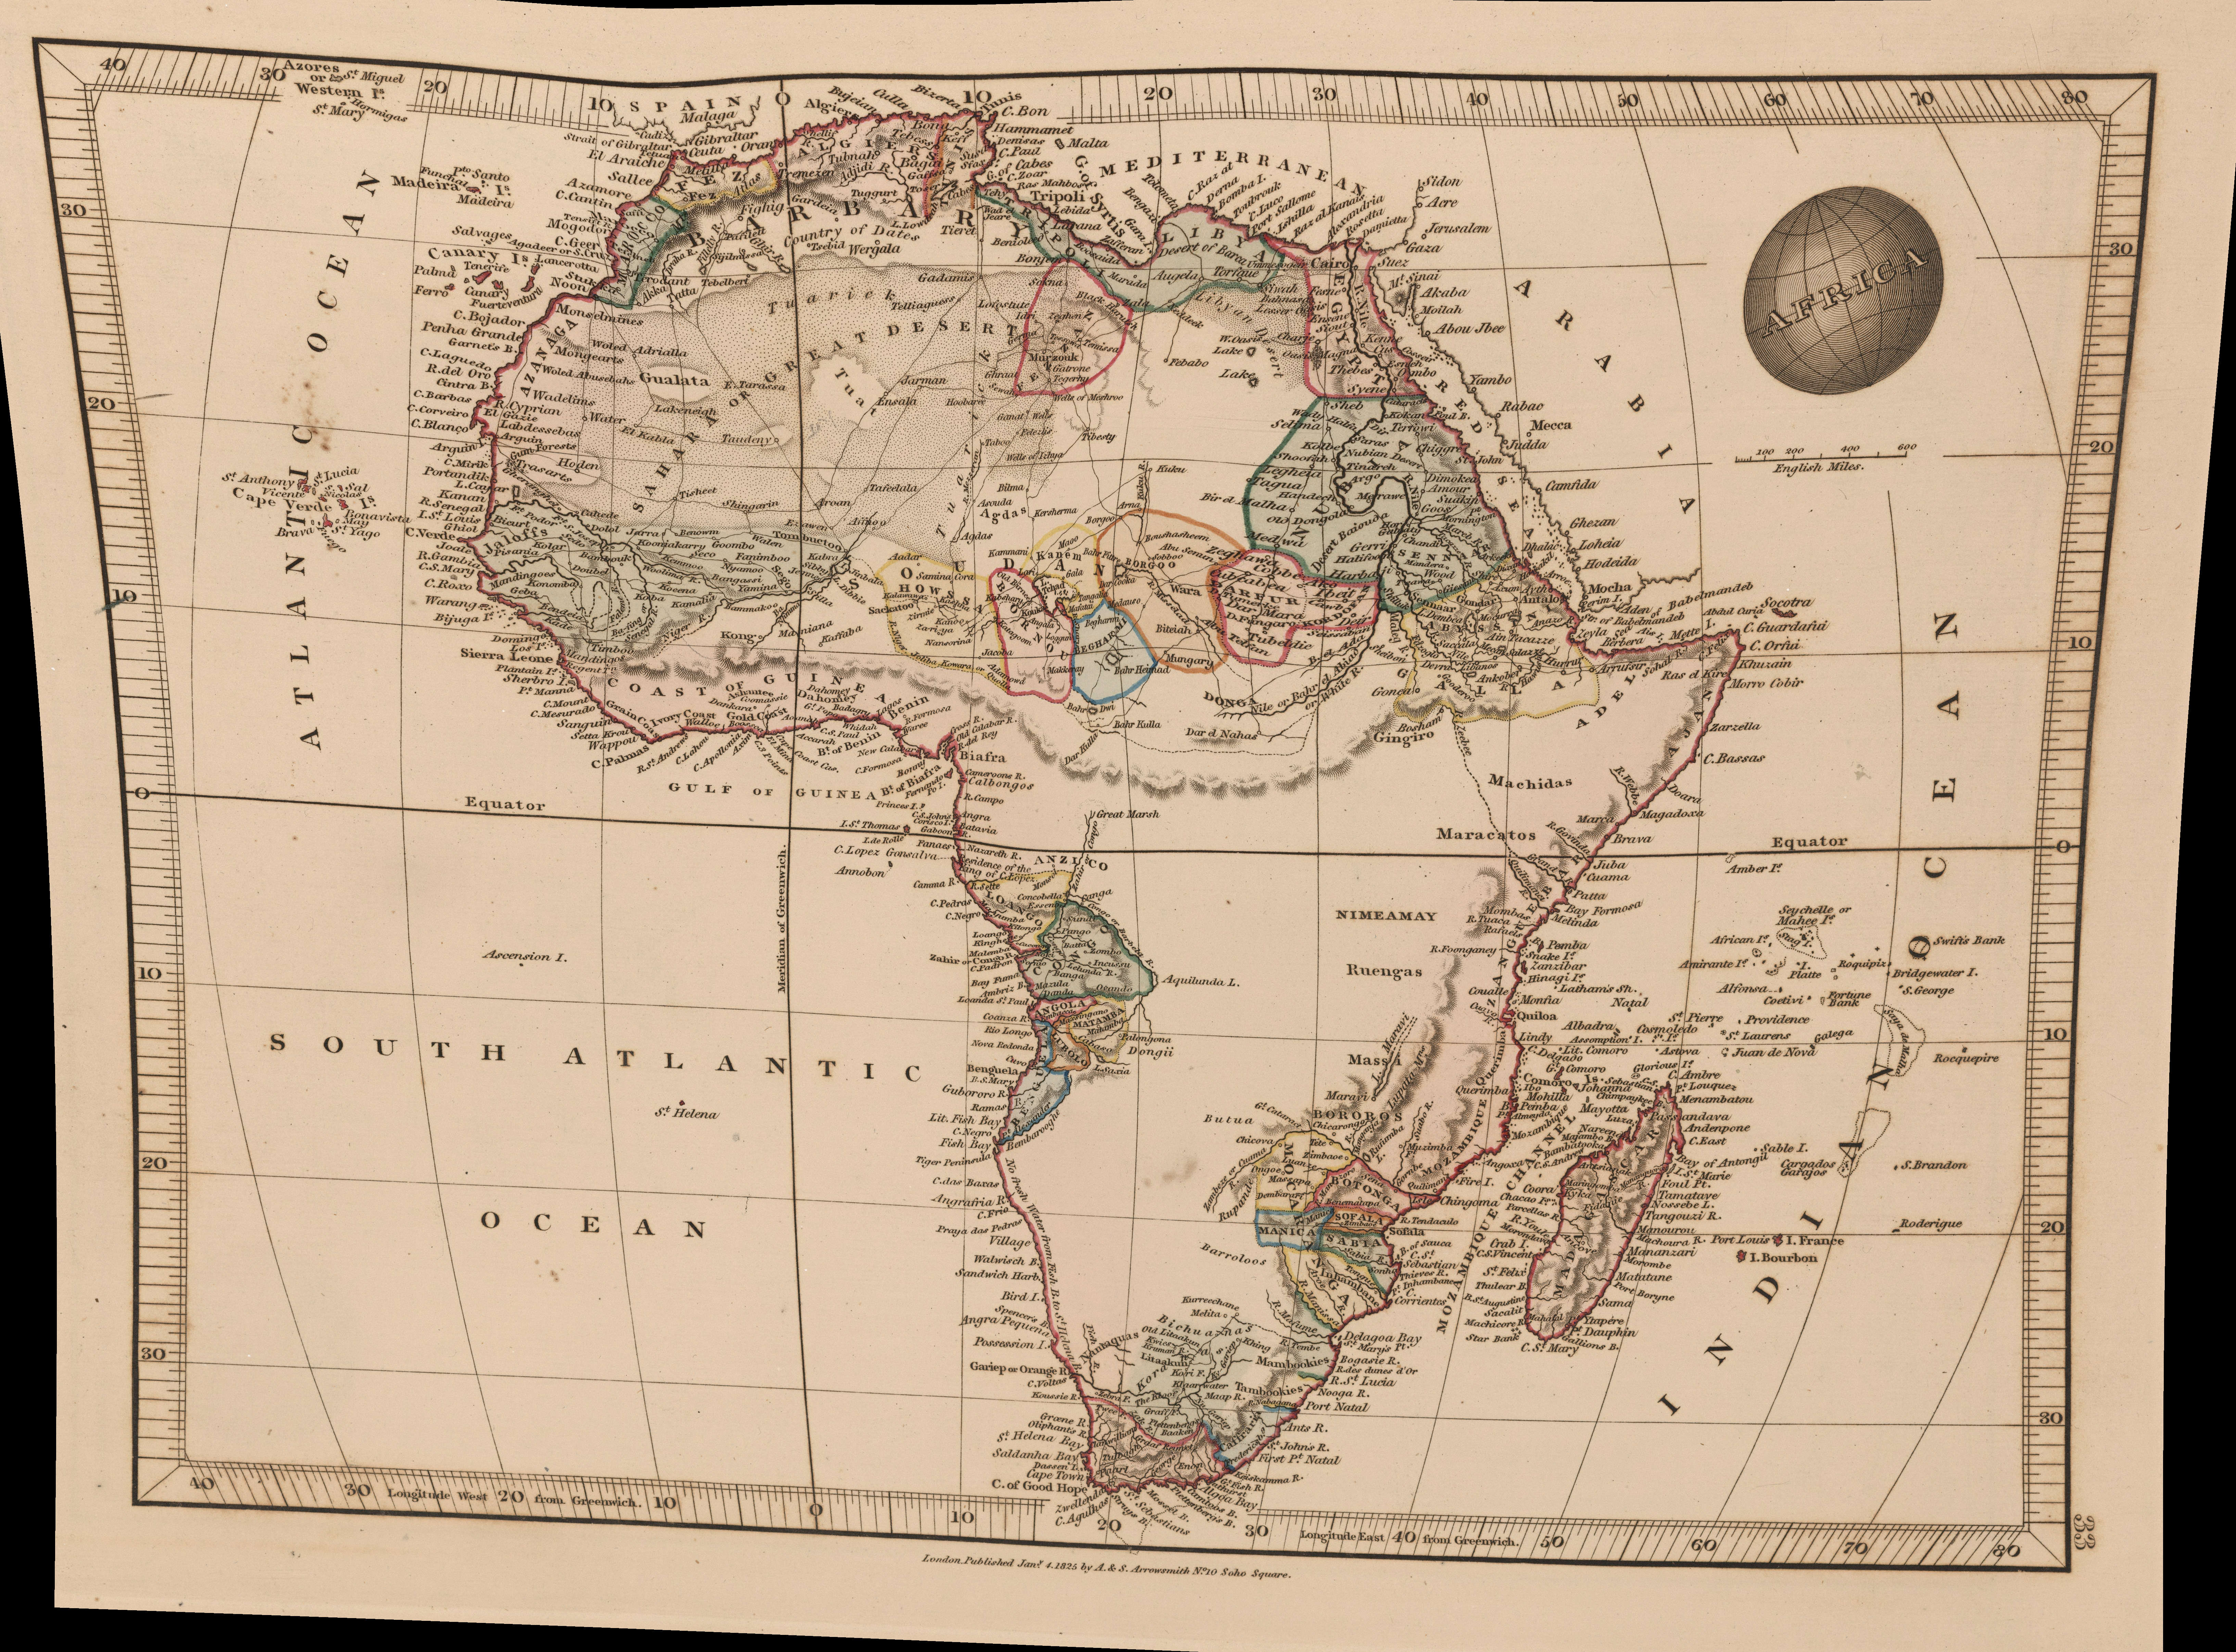
\includegraphics[width=0.8\linewidth]{img/Arrowsmith.jpg}
	\caption{Example of georeferenced map}%
	\label{fig:Arrowsmith}
\end{figure}

%\begin{multicols}{2}

In the end we were left with over 3400 polygons (state-shape-years) covering the
period 1800 to 1914 for continental Africa and Madagascar. For some pre-colonial
states in the ISD there were no maps for any years, some are covered only for
some of the years they are in the ISD, but a substantial number of them are
covered by multiple maps for many years. When maps disagreed on where the
various borders were in a given year, we take it as an indication of the
ambiguity of where a given state had \emph{de facto} or \emph{de jure} control
in that year. In the areas where all the maps agree we could be quite sure that
the given state entity had real presence.  While in areas where only one map
indicated that the state was presence, this could either be wrong, an indication
of \emph{de jure} as opposed to \emph{de facto} presence or some other form of
limited presence. The coding process of looking at hundreds of maps strengthened
this initial intuition, and the resulting figures of state presence drawn from
the complete data lends it further credence. On aggregate most maps should agree
on the core areas of a state while the further away from the core fewer maps
would consider the area part of the state. We believe this approximates the real
ambiguities surrounding where states governed and where they did not, resulting
in a measure of state presence in a given area. Figure \ref{overlay} is an
overlay of all the map polygons of Libya, Tunisia and Egypt. It demonstrates how
the authority of these states faded into the desert, partially overlap at the
borders, and in the Libyan case, its tenuous hold on the Fezzan region. Although
to a lesser degree, one can also see that Libya as a whole spent fewer years as
an independent state than its neighbours in the region.

%\end{multicols}

\begin{figure}[htpb]
	\centering
	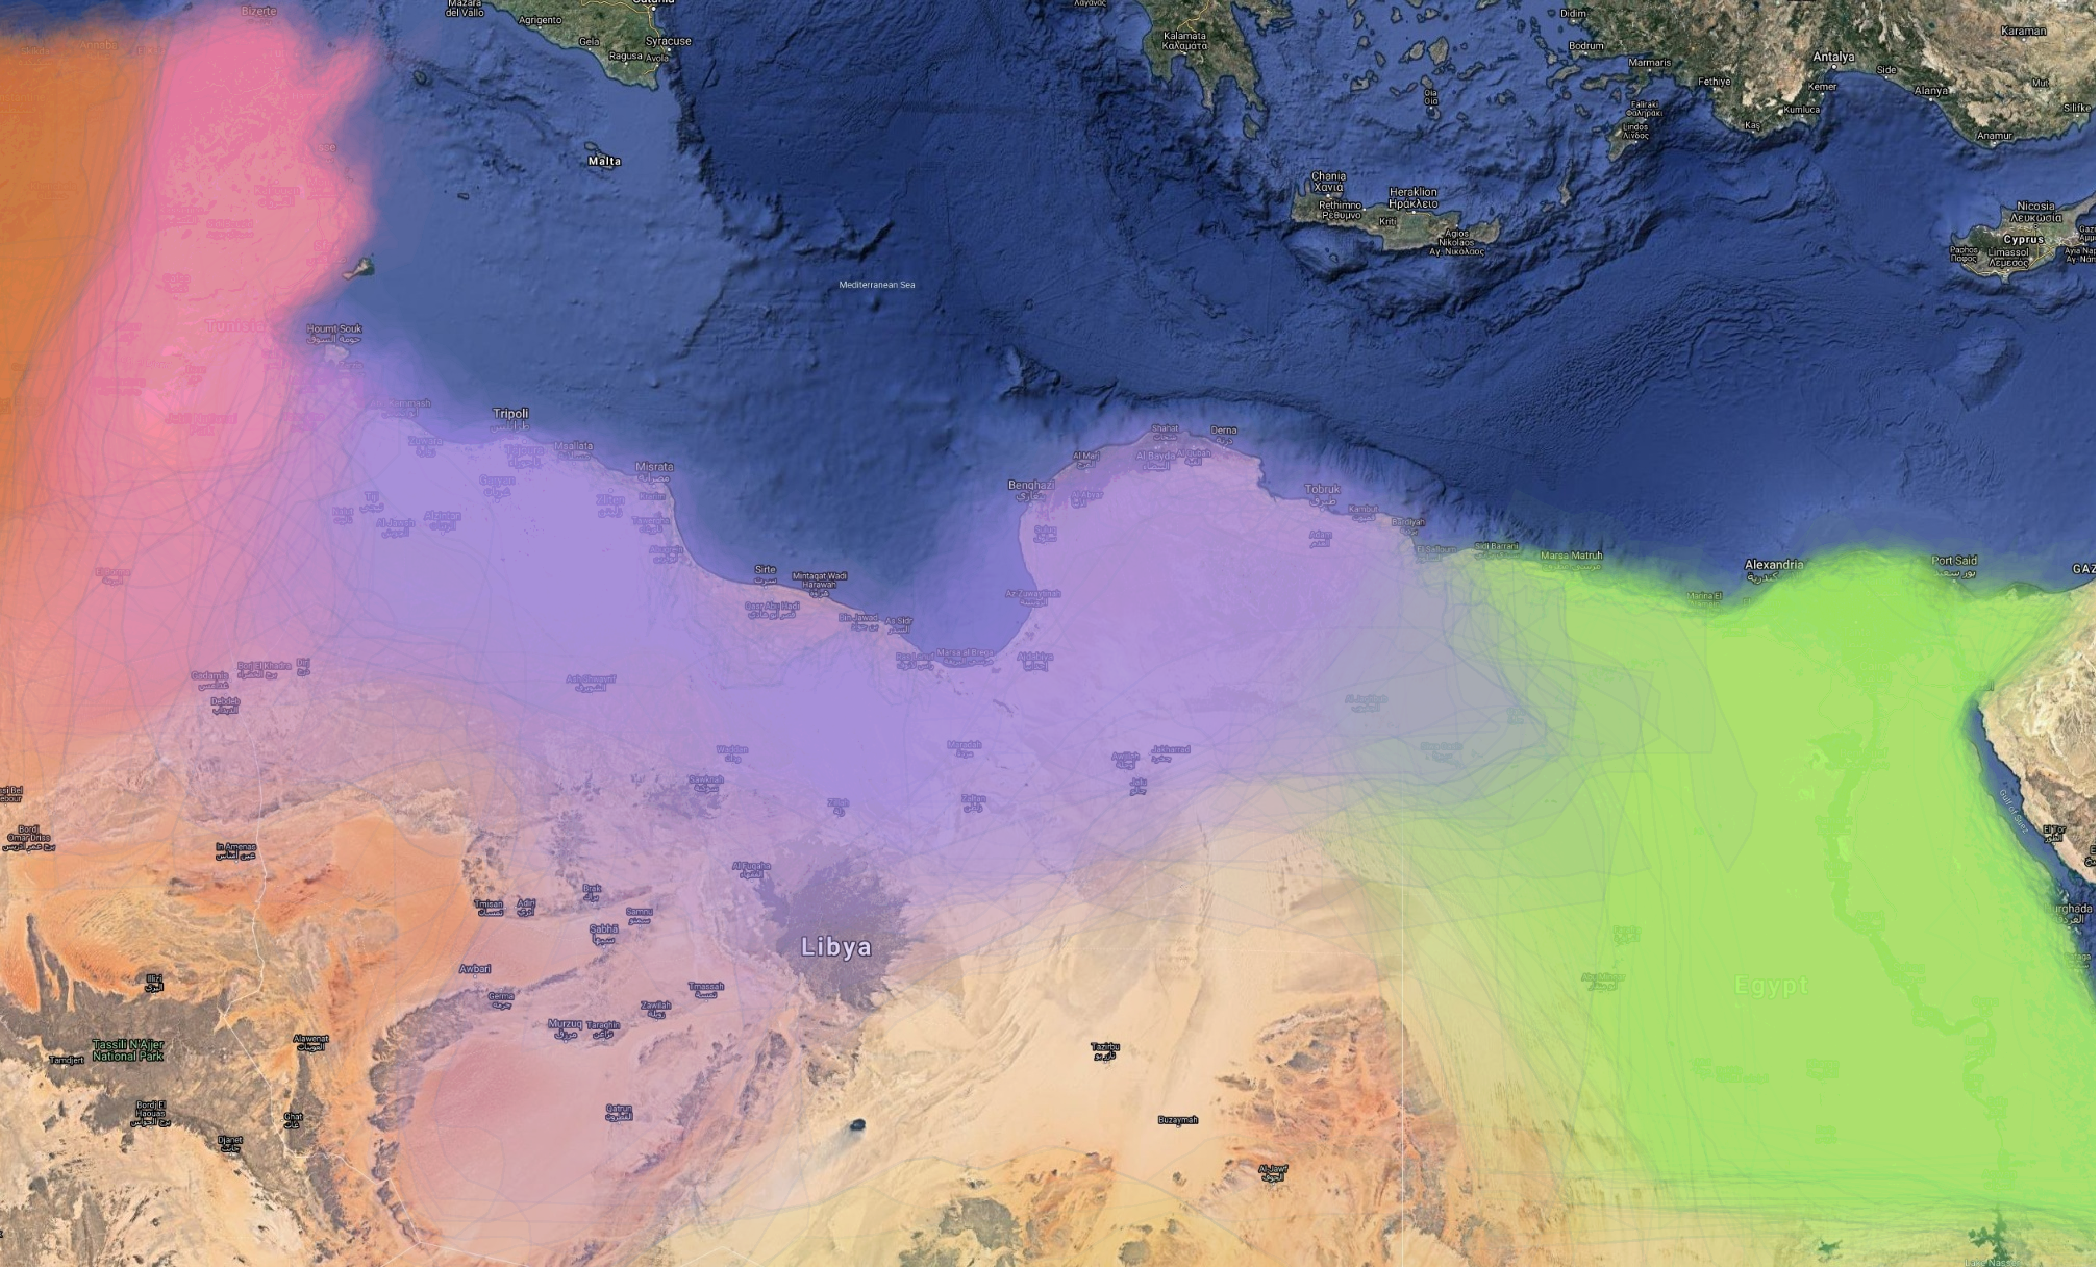
\includegraphics[width=0.8\textwidth,keepaspectratio]{img/TUNLIBEGY.pdf}
	\caption{Overlay of all map polygons of Tunisia, Libya and Egypt}
	\label{overlay}
\end{figure}

%\begin{multicols}{2}

The data from this project can be aggregated and used in multiple ways and to
produce different variables and measures. All of these indicators are aggregated
over all years for individual PRIO-GRID cells in Africa. The primary indicator
used in this paper is a measure of the presence over time. It is measured by the
number of maps that indicate that a state was present there, counting only those
of the state most often present in that cell. So that if a cell bordering
Tunisia and Libya contains 40 maps of Tunisia and 7 maps of Libya, only the
Tunisian maps are counted. Including the Libyan maps would risk over counting as
it most likely does not represent additional state presence, but rather
overlapping state presence. 

%\end{multicols}

\begin{figure}[htpb]
	\centering
	%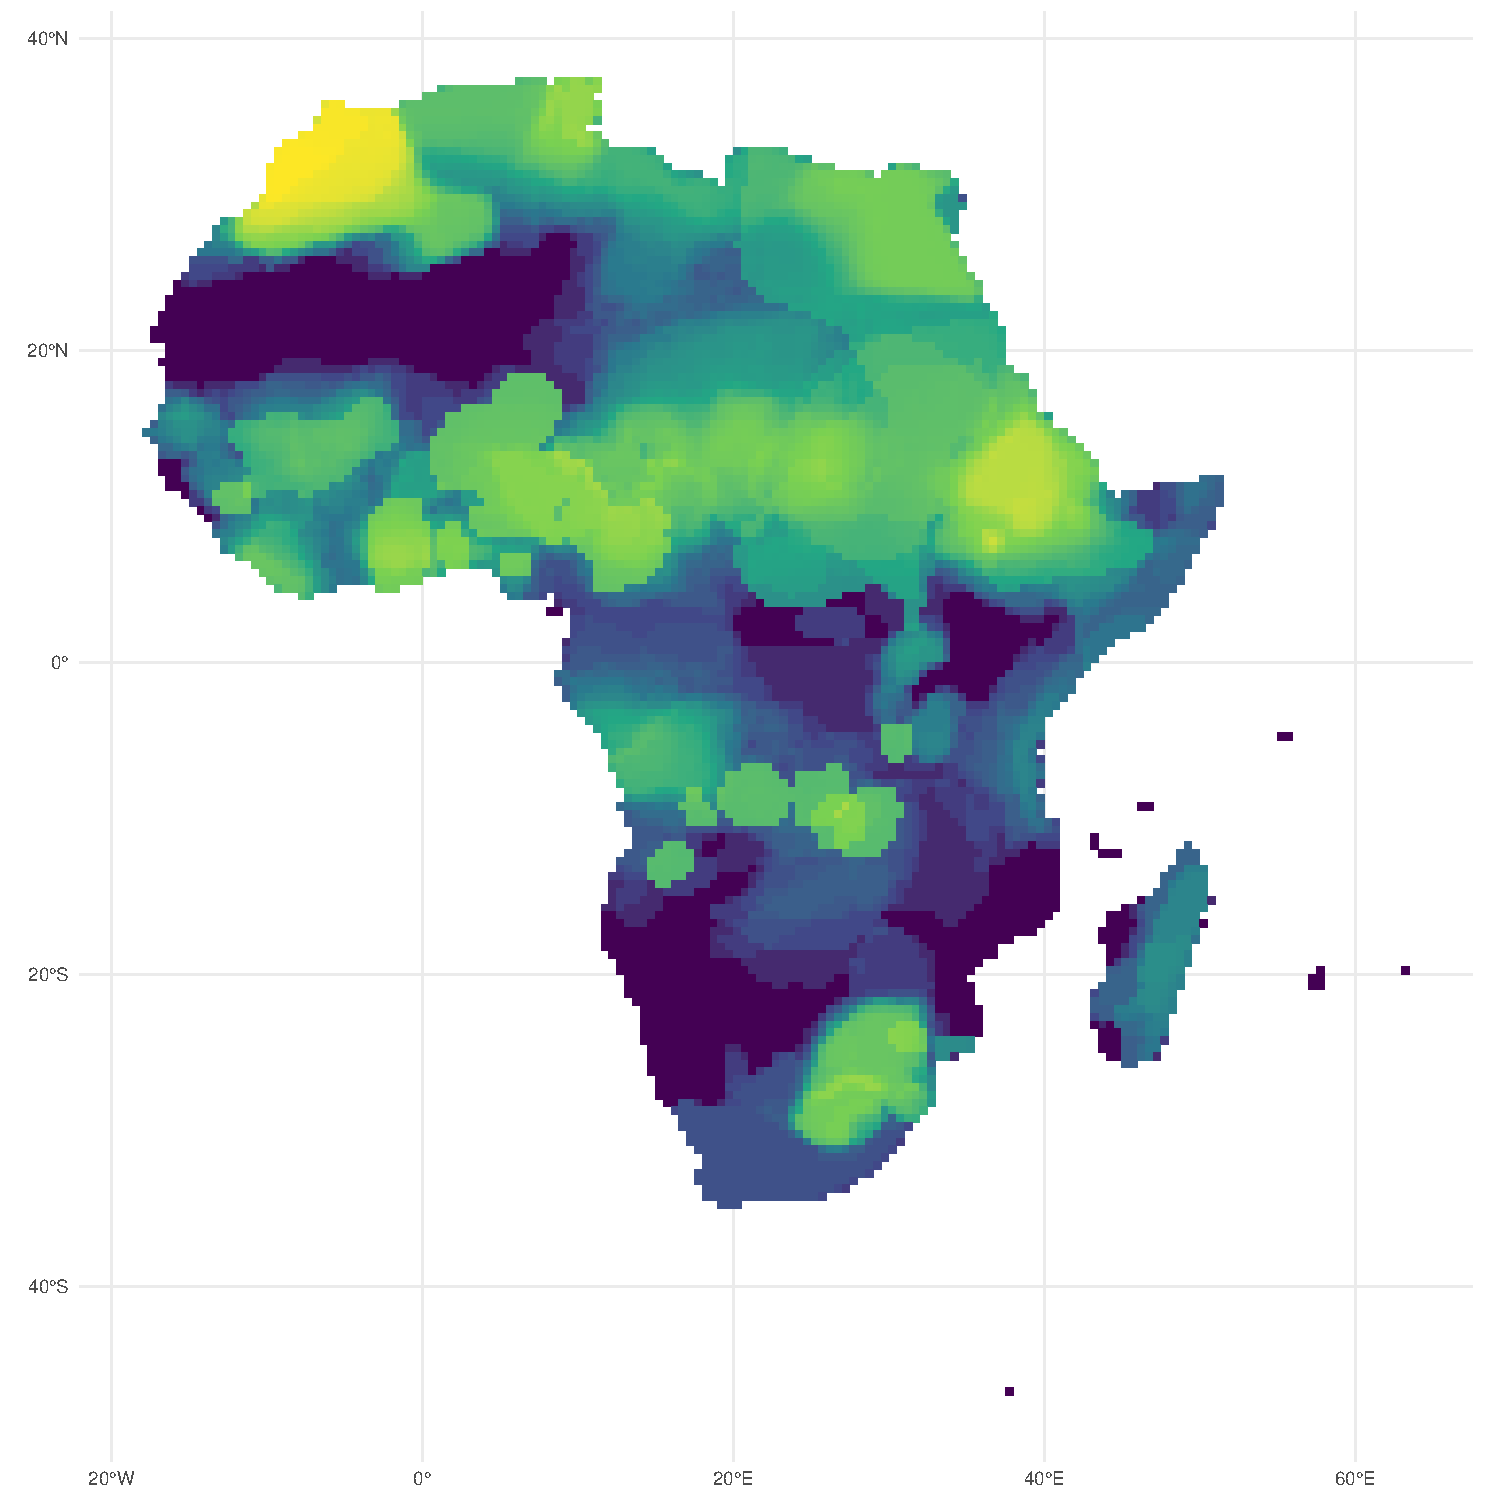
\includegraphics[width=0.8\linewidth]{../Rplot_ln_sp_int.pdf}
	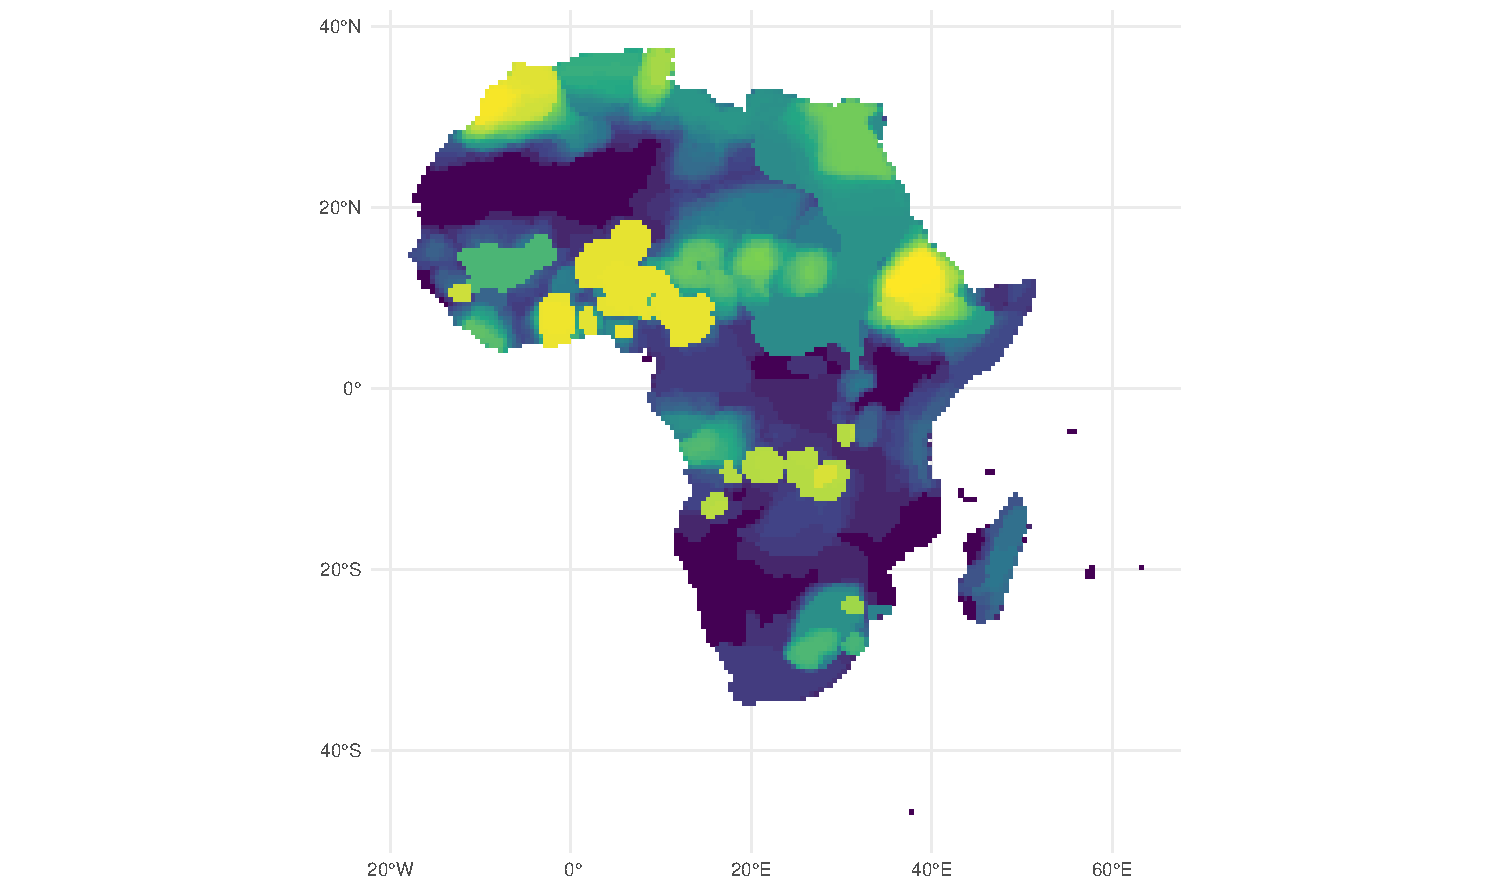
\includegraphics[width=\linewidth]{../R/Output/sp_os_i_sum_any_plot.pdf}
	\caption{State presence (sqrt transformed) with interpolated years based
	on historical atlases.}
	\label{Sp_i}
\end{figure}

\begin{figure}[htpb]
	\centering
	%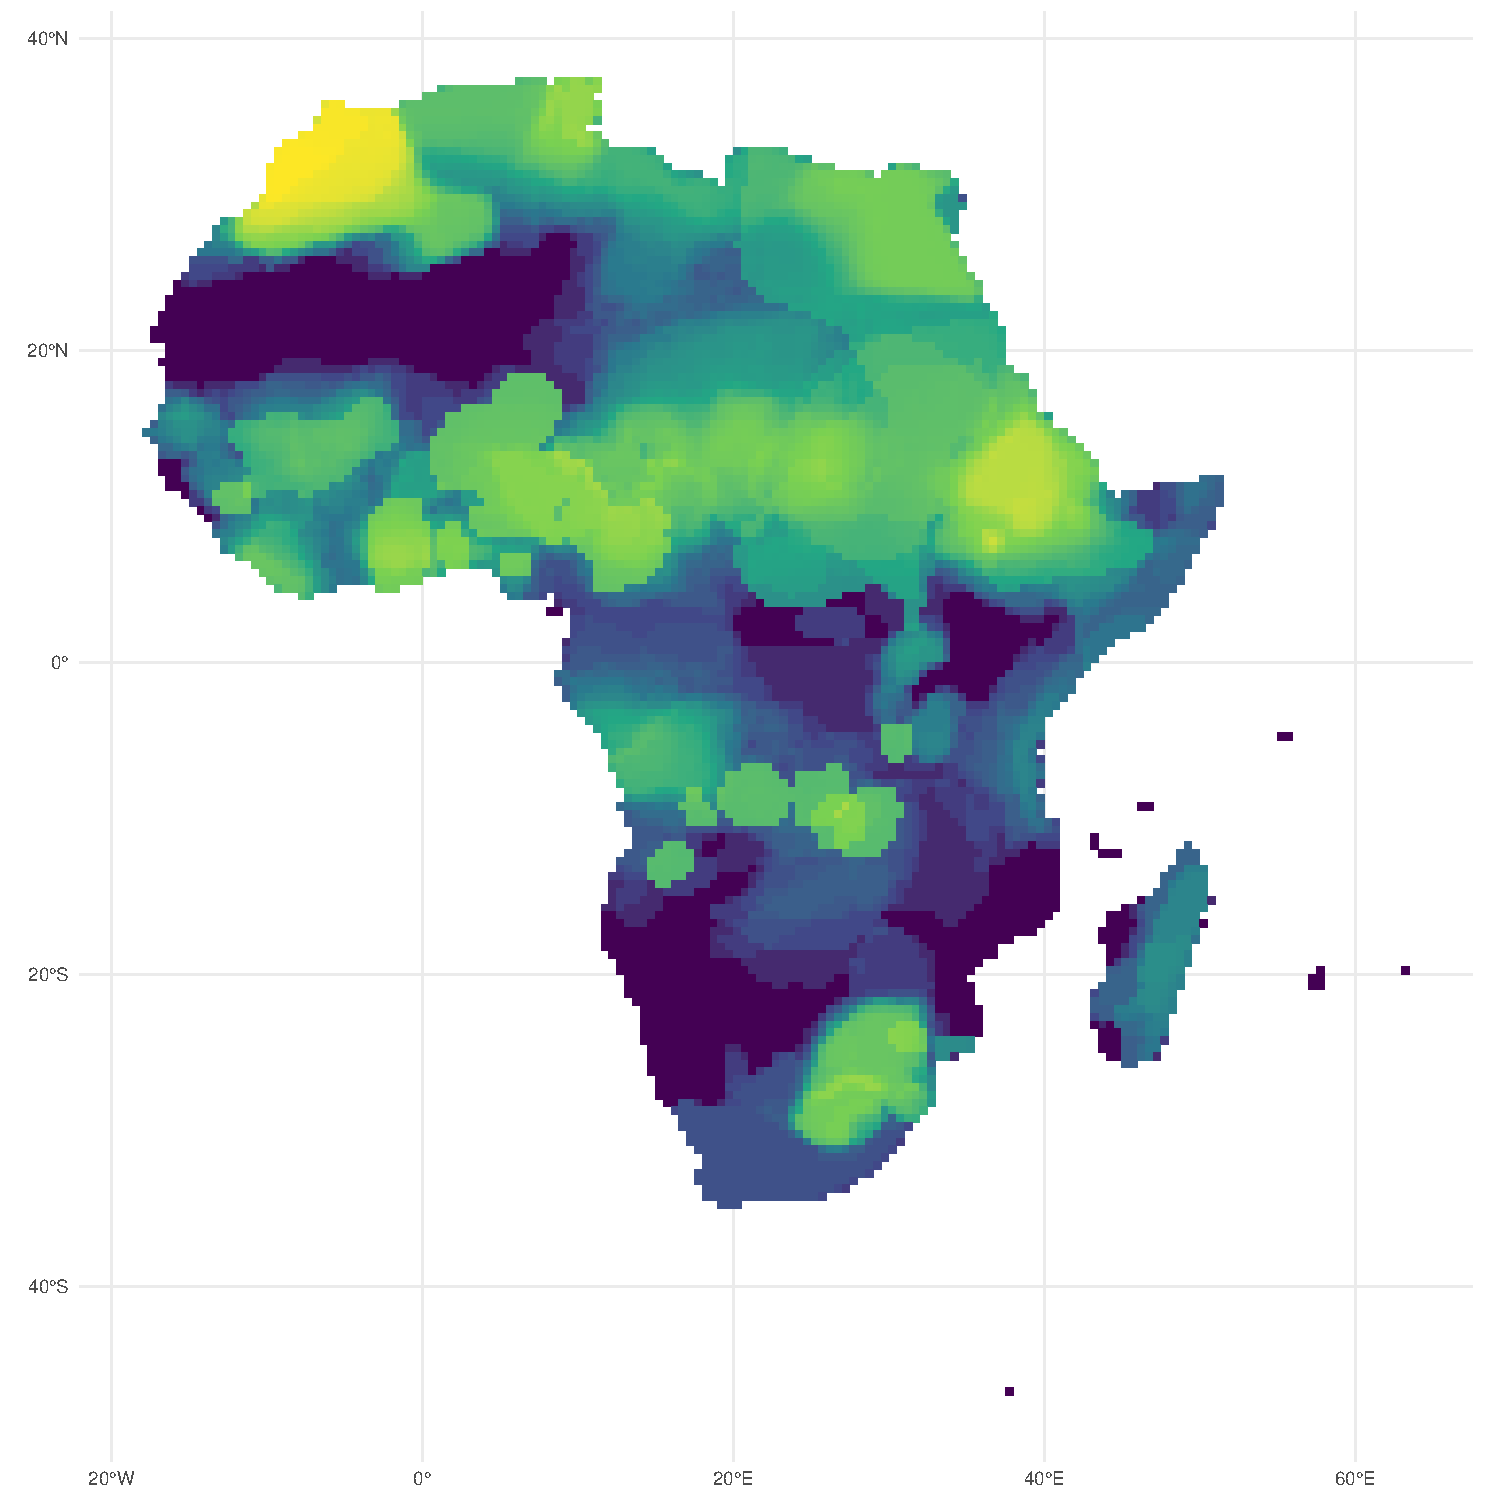
\includegraphics[width=0.8\linewidth]{../Rplot_ln_sp_int.pdf}
	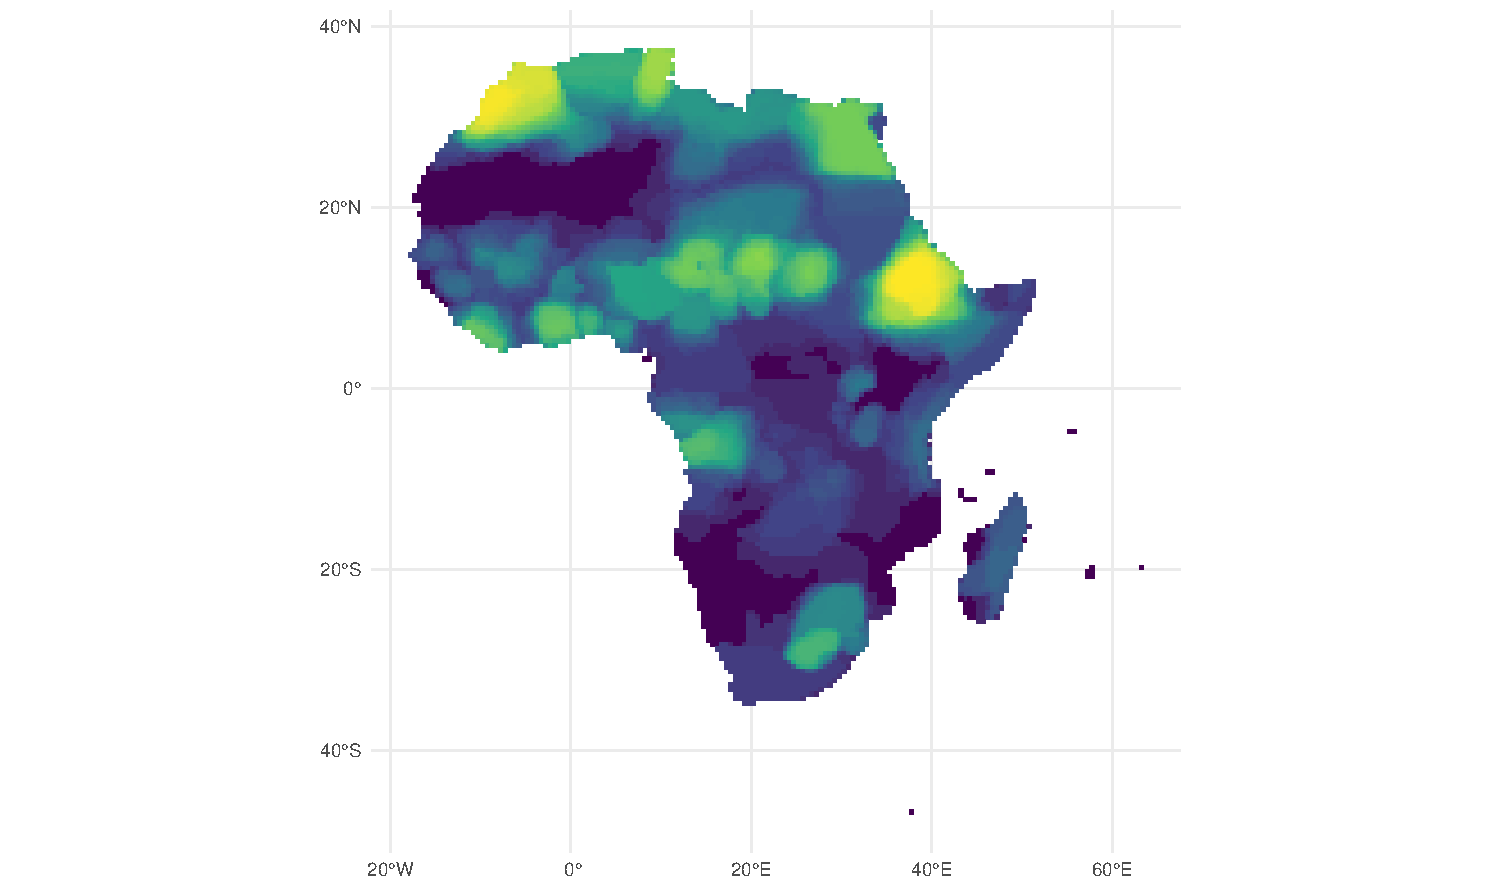
\includegraphics[width=\linewidth]{../R/Output/sp_os_sum_any_plot.pdf}
	\caption{State presence (sqrt transformed)}
	\label{Sp}
\end{figure}

%\begin{multicols}{2}

\section{Research design}

\subsection{Dependent variable}

The unit of analysis are PRIO grid cells, which are one degree by one degree
cells \citep{Tollefsen2012}. Due to the explanatory variable being
time-invariant, the analysis is limited to a cross section. Accordingly, the
dependent variables are fatalities and the number of state based conflict events
per grid cell in the period 1946-2018 *** Check end date ***. In other words
these are cross sectional count data. The data are from the GED project
\citep{Sundberg2013}.

% Run models excluding org3 events and fatalities, citing my other paper?

\subsection{Independent variable}

The main explanatory variable is the per grid cell sum of state presence. For
the main model I use measure of state presence from the Geo-ISD that counts all
maps that intersect a given grid cell, even if multiple maps do so in a single
year, but only for the state that has the most presence overall in that grid
cell. This measure has the benefit of including more data, which allows for the
approximation of relative degrees of state presence by one state in any year, as
described in the data section above. At the same time it avoids over counting
state presence where there were overlaps in sovereignty or changes in who
controlled the territory. As a robustness check I also ran models using the
measure that counts if there was any state presence in a grid-cell-year (as a
yearly dummy). In other words, this could be at most 214, and it is more so a
measure of the maximum \textit{extent} of state presence, and is less accurate
in terms of depth. The benefit of this measure is that it avoid the potential
over representation of countries frequently mapped by Europeans, such as the
North African states (proximity) and Darfur (weird obsession?) Again counting
only the presence of the most present state for each grid cell. In both cases
this paper uses the measure which includes interpolated shapes from historical
atlases. Where historical atlases depicted the borders of a state from year x to
y, we created identical shapes for all these years. This has the benefit of
placing a slightly larger emphasis on the historical atlases, at the cost of
being static.\footnote{Equivalent models excluding the interpolated shapes are
included in the Online appendix. Results remain substantially the same for all
specifications.}

\subsection{Controls}

Mountains help in early state formation by providing protection and limiting the
exit options of sedentary farmers \citep{Carneiro1988}. Mountainous terrain has
also been linked with civil conflict by providing shelter for rebel groups
\citep{Hegre2006}, although this relationship is debated 
\citep{Buhaug2002}. The data is from the PRIO-grid data set, but originally 
from \citet{Blyth2002}. 

Water is essential for state formation. States typically formed either as
coastal cities, close to navigable rivers or by the shores of great lakes.
People still tend to live next to a source of water, thus this acts as a proxy
for population density, and fighting usually happens where there are people.
Water could also be related to the conflict measures more directly by being a
non divisible resource to fight for control over. *** SOURCES NEEDED ***. The
data on water as a percentage of the grid surface is from the PRIO-grid data
set, but originally from the European Space Agency \citep{Bontemps2009}.

Distance to coast could affect both state presence and conflict in a number of
ways. First, as state above, states were more likely to be formed along the
coast as it connected cities and people. A special case for Africa is also the
existence of slave raiding/trading states that formed along the eastern and
western coasts of the continent. These states raison d'être was raiding slaves
from tribes and peoples inland and selling them to coastal traders (European in
the West and Arab in the east). \citet{Nunn2008} argues that this state of
affairs left legacies of mistrust and antagonism, which has resulted in
increased levels of current day conflict. Distance to the coast could also be
related to the measure of state presence through the fact that our measure is
based on European observations (maps), which undoubtedly had better coverage
along the coast, especially for the earlier periods. Distance to the coast could
further be related to conflict through lower levels of development. The distance
to coast data is from the PRIO-grid data set, but originally from *** INSERT
SOURCE ***.

Barren terrain could correlate with both state presence and conflict by 

Population density could be a consequence of prior state building and could
correlate with conflit measures as fighting broadly speaking happens where there
are at least some population. I therefor include an estimate of population
density in *** INSERT YEAR *** from the HYDE project \citep{Goldewijk2016}.
Because this is an estimate and not a measurement, I also include a measure of
the barrenness of each grid cell from the PRIO-grid data set, but originally
from *** INSERT SOURCE ***. This measure proxies population density because
people generally do not live on barren land, and captures the large amount of
zeroes in both the Sahara and Kalahari deserts.

As a robustness check some models also include measures of temperature (mean and
variance), precipitation (mean and variance) and forest (remove?), as these have
been found to affect conflict and could potentially affect state building ***
Ask Ole Magnus about these, I don't see the connection ***

Distance to borders *** Put back in ***. Could be related to state presence
because despite their reputation African borders were not drawn completely at
random (or along meridian lines). For example, the borders of northern Nigeria
and Niger were based on the extent of the Sokoto Caliphate and the neighboring
Kanem-Bornu (or just Bornu) empire \citep{HiribarrenVincent2017AHoB}. Proximity
to international border has also been found to predict conflict
\citep{Buhaug2002}. I use the measure included in the PRIO grid data, which is
originally from *** ISERT SOURCE ***.

\subsection{Alternative measures}

*** So far I have none ***

\subsection{Modelling}

My main models are negative binomial models to account for the dependent
variable being count data (count of deaths (fatalities) and count of conflict
events (state based)). *** As I currently understand the assumptions of it, I
should not have to transform the data, as I have done (in the results presented
below), as the negative binomial model accounts for the non-linear nature of the
data. ***

TODO: To fitness test for whether negative binomial or Poisson regression is
most appropriate. I suspected it would be negative binomial, so I went with
that, but this needs to be confirmed.

Zero inflated negative binomial is probably a good idea. Zeros could be true
zeros - there were no fatalities or state based conflict events in the grid cell
during the period, or zeros could be measurement error, most likely resulting
from lack of reporting. However, I am not familiar with ZIMB models at this
point, but I will figure it out before the next draft.

I should also probably be controlling for spatial interdependence, but again, I
am not yet familiar with the method of doing so. Will be addressed in future
versions.

\section{Preliminary results}

I have run a whole lot of model specifications, some of which are reported below
in the figures and in the tables in the appendix. The positive relationship
between state presence and conflict is as surprising as it is robust across all
models. The results of the interaction models might help explain the
relationship. As seen in Figure \ref{deaths_int} and Figure \ref{sb_int}, state
presence is negatively correlated with both conflict measure close to the
capital, but becomes positive and significant further away from the capital.
This supports an interpretation that state presence can be conflict reducing in
those cases where it makes a country less artificial for all the reasons
outlined by the conflict reducing arguments in the literature. Taken tougher
however, the results indicate that the negative effects of higher values of
state presence further away form the capitals of Africa outweighs these conflict
reducing effects. 

%\end{multicols}

\begin{figure}[htpb]
	\centering
	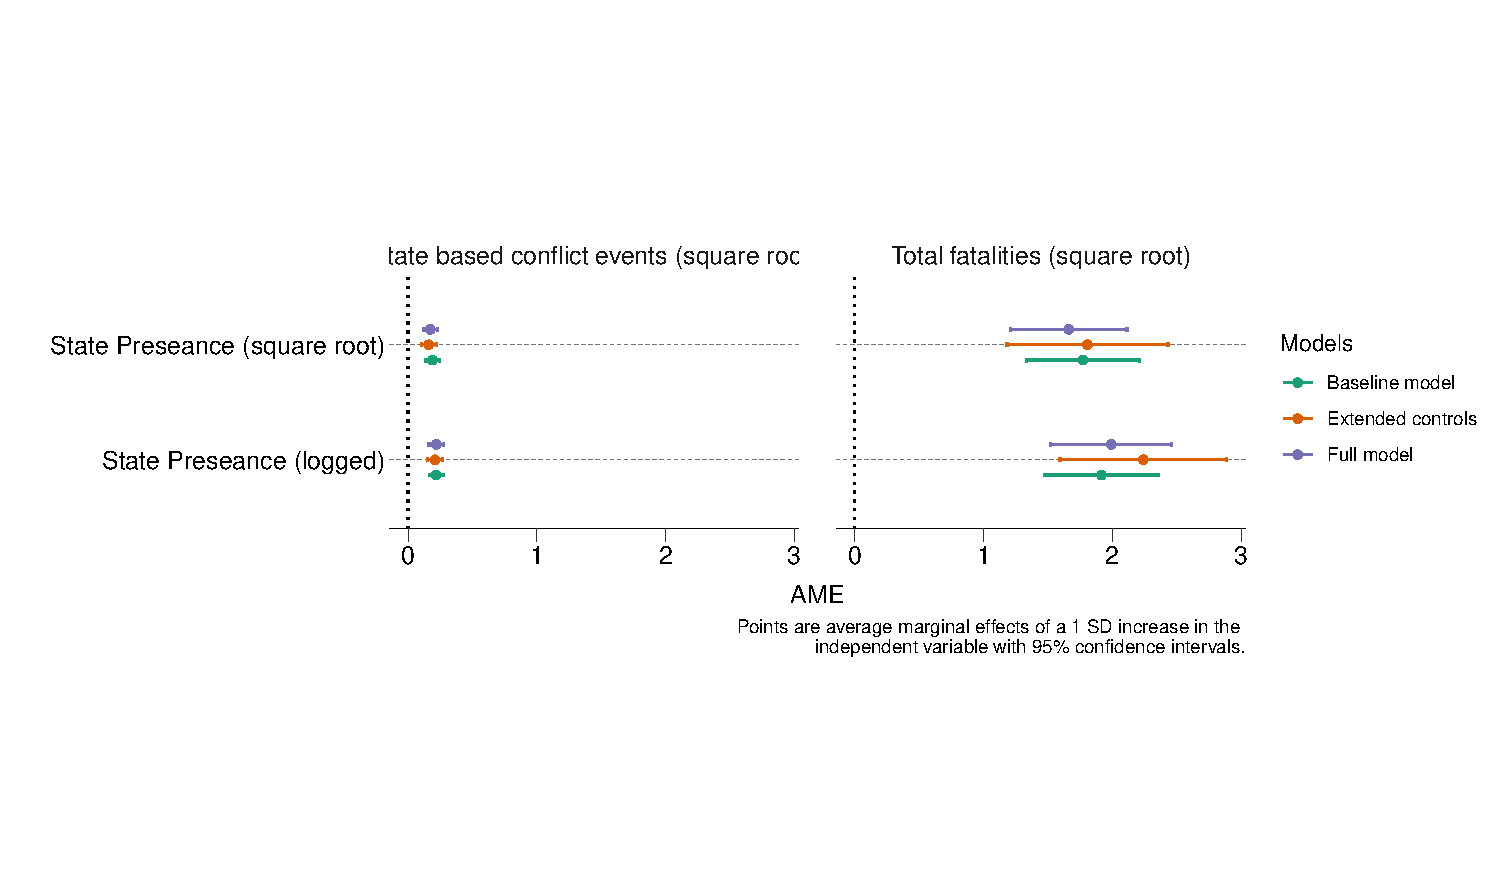
\includegraphics[width=\linewidth]{"../R/Output/conflictMargins.pdf"}
	\caption{}
	\label{margins}
\end{figure}

\begin{figure}[htpb]
	\centering
	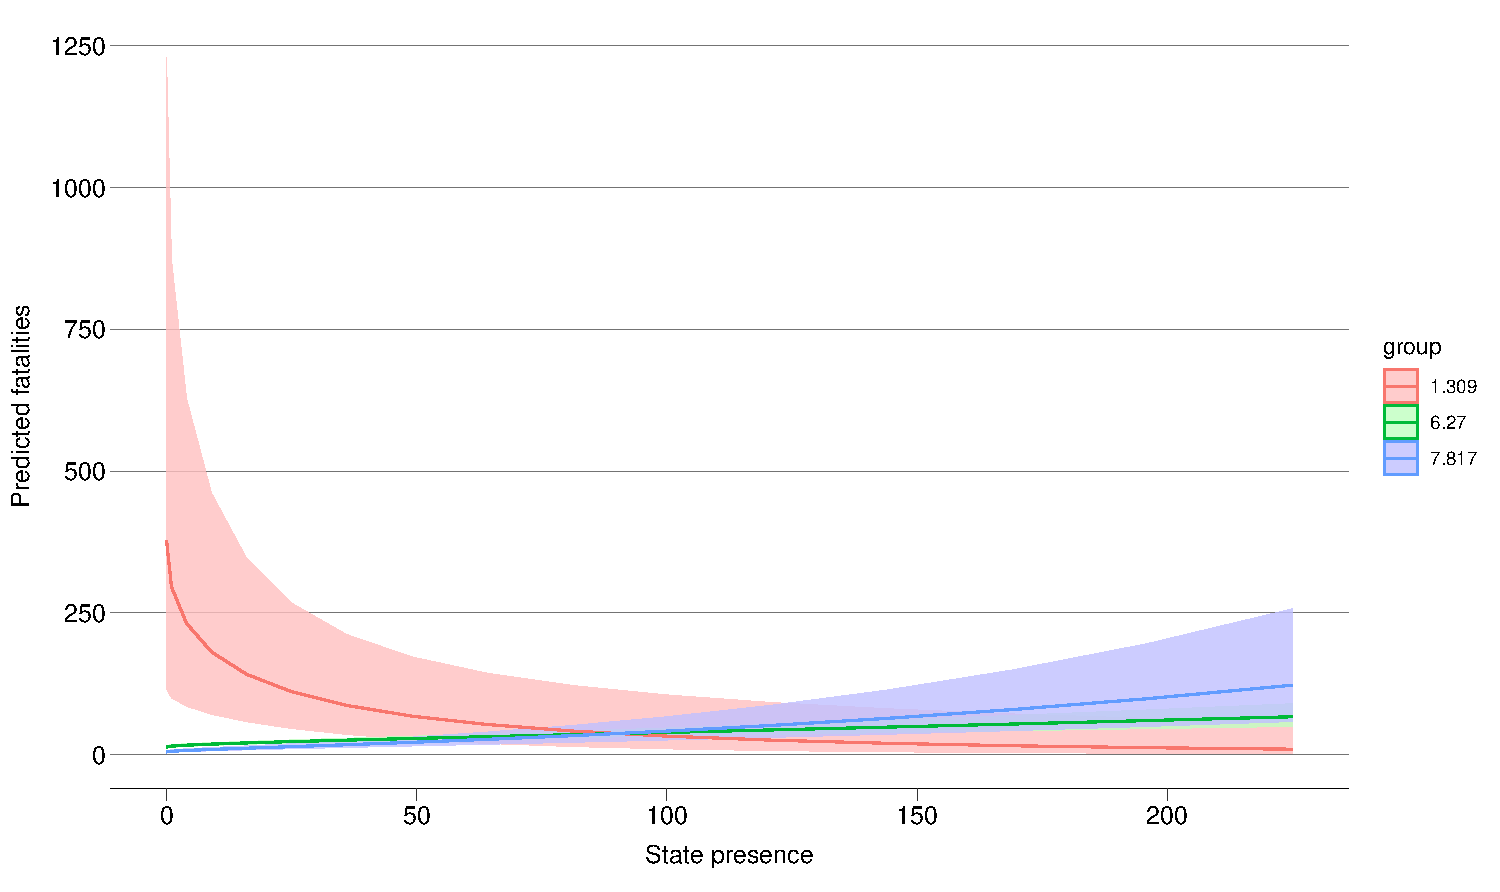
\includegraphics[width=\linewidth]{"../R/Output/deathsIntPlot.pdf"}
	\caption{}
	\label{deaths_int}
\end{figure}

\begin{figure}[htpb]
	\centering
	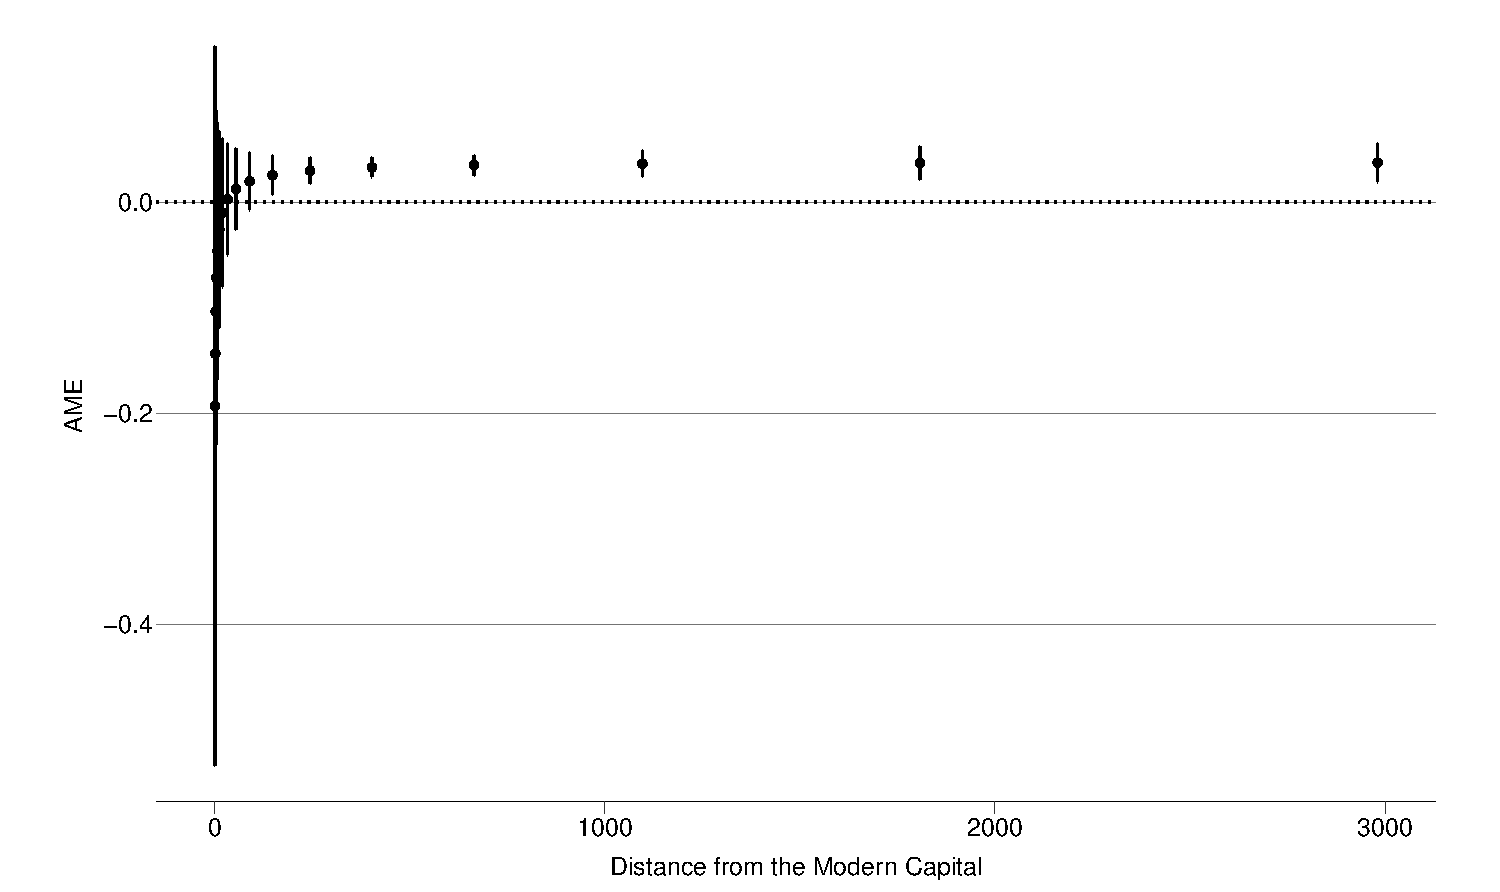
\includegraphics[width=\linewidth]{"../R/Output/state_based_int_plot.pdf"}
	\caption{}
	\label{sb_int}
\end{figure}

%\begin{multicols}{2}

\section{Conclusion}

*** Awaiting more detailed results ***

%\end{multicols}

\pagebreak

\bibliographystyle{agsm}
\bibliography{../lib.bib}

\pagebreak
\section*{Appendix}


\begin{sidewaystable}
\begin{center}
\scalebox{1}{
\begin{tabular}{l c c c c c c}
\hline
 & Baseline & Extended Controls & Baseline & Extended Controls & Baseline & Extended Controls \\
\hline
(Intercept)     & $3.26^{***}$  & $2.29^{***}$  & $3.65^{***}$  & $2.63^{***}$  & $4.07^{***}$  & $2.95^{***}$  \\
                & $(0.13)$      & $(0.14)$      & $(0.12)$      & $(0.13)$      & $(0.11)$      & $(0.13)$      \\
logSpAll        & $0.30^{***}$  & $0.28^{***}$  &               &               &               &               \\
                & $(0.03)$      & $(0.03)$      &               &               &               &               \\
mountains\_mean & $2.36^{***}$  & $1.24^{***}$  & $2.29^{***}$  & $1.08^{***}$  & $2.21^{***}$  & $1.09^{***}$  \\
                & $(0.19)$      & $(0.19)$      & $(0.19)$      & $(0.19)$      & $(0.20)$      & $(0.19)$      \\
water\_gc       & $0.02^{***}$  & $0.01^{***}$  & $0.03^{***}$  & $0.01^{***}$  & $0.02^{***}$  & $0.01^{***}$  \\
                & $(0.00)$      & $(0.00)$      & $(0.00)$      & $(0.00)$      & $(0.00)$      & $(0.00)$      \\
barren\_gc      & $-0.03^{***}$ & $-0.02^{***}$ & $-0.03^{***}$ & $-0.02^{***}$ & $-0.03^{***}$ & $-0.02^{***}$ \\
                & $(0.00)$      & $(0.00)$      & $(0.00)$      & $(0.00)$      & $(0.00)$      & $(0.00)$      \\
distcoast       & $0.00^{***}$  & $0.00^{***}$  & $0.00^{***}$  & $0.00^{***}$  & $0.00^{***}$  & $0.00^{***}$  \\
                & $(0.00)$      & $(0.00)$      & $(0.00)$      & $(0.00)$      & $(0.00)$      & $(0.00)$      \\
logPopd         &               & $1.03^{***}$  &               & $1.03^{***}$  &               & $1.05^{***}$  \\
                &               & $(0.07)$      &               & $(0.07)$      &               & $(0.07)$      \\
bdist3          &               & $-0.00^{*}$   &               & $-0.00^{*}$   &               & $-0.00^{*}$   \\
                &               & $(0.00)$      &               & $(0.00)$      &               & $(0.00)$      \\
sqrtSpAll       &               &               & $0.10^{***}$  & $0.09^{***}$  &               &               \\
                &               &               & $(0.01)$      & $(0.01)$      &               &               \\
SpAll10         &               &               &               &               & $0.00^{***}$  & $0.00^{***}$  \\
                &               &               &               &               & $(0.00)$      & $(0.00)$      \\
\hline
AIC             & $43066.10$    & $42817.43$    & $43101.68$    & $42851.53$    & $43143.35$    & $42890.13$    \\
BIC             & $43116.91$    & $42882.75$    & $43152.48$    & $42916.85$    & $43194.16$    & $42955.45$    \\
Log Likelihood  & $-21526.05$   & $-21399.71$   & $-21543.84$   & $-21416.77$   & $-21564.67$   & $-21436.07$   \\
Deviance        & $5340.87$     & $5355.31$     & $5338.89$     & $5353.37$     & $5336.65$     & $5351.13$     \\
Num. obs.       & $10492$       & $10482$       & $10492$       & $10482$       & $10492$       & $10482$       \\
\hline
\multicolumn{7}{l}{\scriptsize{$^{***}p<0.001$; $^{**}p<0.01$; $^{*}p<0.05$; $^{\cdot}p<0.1$}}
\end{tabular}
}
\caption{Fatalities}
\label{deaths}
\end{center}
\end{sidewaystable}


\begin{sidewaystable}
\begin{center}
\scalebox{1}{
\begin{tabular}{l c c c c}
\toprule
 & Geography & North Africa & Population densisty & Distance
		  to border \\
\midrule
Precolonial state presence (sqrt)        & $0.07^{***}$  & $0.05^{***}$  & $0.04^{***}$  & $0.04^{***}$    \\
                                         & $(0.01)$      & $(0.01)$      & $(0.01)$      & $(0.01)$        \\
Precolonial state presence (sqrt)        & $0.07^{***}$  & $0.05^{***}$  & $0.04^{***}$  & $0.04^{***}$    \\
                                         & $(0.01)$      & $(0.01)$      & $(0.01)$      & $(0.01)$        \\
Mountainous terrain                      & $0.87^{***}$  & $0.81^{***}$  & $-0.22$       & $-0.28^{\cdot}$ \\
                                         & $(0.16)$      & $(0.16)$      & $(0.15)$      & $(0.15)$        \\
Water (\%)                               & $-0.01^{*}$   & $-0.01^{*}$   & $-0.01^{**}$  & $-0.01^{***}$   \\
                                         & $(0.00)$      & $(0.00)$      & $(0.00)$      & $(0.00)$        \\
Barren (\%)                              & $-0.02^{***}$ & $-0.02^{***}$ & $-0.01^{***}$ & $-0.01^{***}$   \\
                                         & $(0.00)$      & $(0.00)$      & $(0.00)$      & $(0.00)$        \\
Distance to coast (log)                  & $-0.16^{***}$ & $-0.14^{***}$ & $-0.11^{***}$ & $-0.08^{***}$   \\
                                         & $(0.02)$      & $(0.02)$      & $(0.02)$      & $(0.02)$        \\
Population density (log)                 &               &               & $1.00^{***}$  & $0.94^{***}$    \\
                                         &               &               & $(0.06)$      & $(0.06)$        \\
Distance to international boundary (log) &               &               &               & $-0.20^{***}$   \\
                                         &               &               &               & $(0.04)$        \\
North Africa                             &               & $0.51^{***}$  & $0.38^{**}$   & $0.47^{***}$    \\
                                         &               & $(0.13)$      & $(0.12)$      & $(0.12)$        \\
\midrule
AIC                                      & $20314.22$    & $20297.34$    & $20007.10$    & $19979.16$      \\
BIC                                      & $20364.33$    & $20354.61$    & $20071.52$    & $20050.74$      \\
Log Likelihood                           & $-10150.11$   & $-10140.67$   & $-9994.55$    & $-9979.58$      \\
Deviance                                 & $4106.74$     & $4112.96$     & $4158.66$     & $4164.26$       \\
Num. obs.                                & $9492$        & $9492$        & $9492$        & $9492$          \\
\bottomrule
\multicolumn{5}{l}{\scriptsize{$^{***}p<0.001$; $^{**}p<0.01$; $^{*}p<0.05$; $^{\cdot}p<0.1$}}
\end{tabular}
}
\caption{State based conflict events}
\label{state_based}
\end{center}
\end{sidewaystable}


\begin{sidewaystable}
\begin{center}
\scalebox{1}{
\begin{tabular}{l c c c}
\hline
 & Baseline & Extetended Controls & Full Model \\
\hline
(Intercept)          & $2.84^{***}$   & $1.93^{***}$  & $-0.82$       \\
                     & $(0.45)$       & $(0.45)$      & $(0.52)$      \\
sqrtSpAny            & $-0.06$        & $-0.36^{***}$ & $-0.30^{***}$ \\
                     & $(0.09)$       & $(0.09)$      & $(0.08)$      \\
logCapdist           & $-0.39^{***}$  & $-0.35^{***}$ & $-0.33^{***}$ \\
                     & $(0.07)$       & $(0.07)$      & $(0.07)$      \\
mountains\_mean      & $1.04^{***}$   & $0.65^{***}$  & $1.03^{***}$  \\
                     & $(0.13)$       & $(0.12)$      & $(0.13)$      \\
water\_gc            & $0.01^{***}$   & $0.01^{***}$  & $0.01^{***}$  \\
                     & $(0.00)$       & $(0.00)$      & $(0.00)$      \\
barren\_gc           & $-0.02^{***}$  & $-0.01^{***}$ & $-0.01^{***}$ \\
                     & $(0.00)$       & $(0.00)$      & $(0.00)$      \\
distcoast            & $0.00^{***}$   & $0.00^{***}$  & $0.00^{***}$  \\
                     & $(0.00)$       & $(0.00)$      & $(0.00)$      \\
sqrtSpAny:logCapdist & $0.03^{\cdot}$ & $0.07^{***}$  & $0.06^{***}$  \\
                     & $(0.01)$       & $(0.01)$      & $(0.01)$      \\
logPopd              &                & $0.79^{***}$  & $0.82^{***}$  \\
                     &                & $(0.05)$      & $(0.05)$      \\
temp\_sd             &                &               & $0.86^{***}$  \\
                     &                &               & $(0.10)$      \\
temp                 &                &               & $0.05^{***}$  \\
                     &                &               & $(0.01)$      \\
prec\_sd             &                &               & $0.00$        \\
                     &                &               & $(0.00)$      \\
prec\_gpcc           &                &               & $0.00^{*}$    \\
                     &                &               & $(0.00)$      \\
forest\_gc           &                &               & $0.00$        \\
                     &                &               & $(0.00)$      \\
\hline
AIC                  & $29512.34$     & $29259.38$    & $29035.25$    \\
BIC                  & $29577.67$     & $29331.95$    & $29144.07$    \\
Log Likelihood       & $-14747.17$    & $-14619.69$   & $-14502.63$   \\
Deviance             & $5713.62$      & $5758.34$     & $5778.58$     \\
Num. obs.            & $10492$        & $10482$       & $10453$       \\
\hline
\multicolumn{4}{l}{\scriptsize{$^{***}p<0.001$; $^{**}p<0.01$; $^{*}p<0.05$; $^{\cdot}p<0.1$}}
\end{tabular}
}
\caption{Deaths * Distance to capital}
\label{interaction_sqrtDeaths}
\end{center}
\end{sidewaystable}


\begin{sidewaystable}
\begin{center}
\scalebox{1}{
\begin{tabular}{l c c c}
\hline
 & Baseline & Extetended Controls & Full Model \\
\hline
(Intercept)          & $0.91^{*}$    & $-0.50$        & $-3.62^{***}$   \\
                     & $(0.40)$      & $(0.39)$       & $(0.47)$        \\
sqrtSpAny            & $-0.04$       & $-0.24^{**}$   & $-0.09$         \\
                     & $(0.07)$      & $(0.07)$       & $(0.07)$        \\
logCapdist           & $-0.33^{***}$ & $-0.18^{**}$   & $-0.12^{\cdot}$ \\
                     & $(0.06)$      & $(0.06)$       & $(0.06)$        \\
mountains\_mean      & $0.58^{***}$  & $0.19^{\cdot}$ & $0.65^{***}$    \\
                     & $(0.11)$      & $(0.11)$       & $(0.12)$        \\
water\_gc            & $0.01^{**}$   & $0.00^{\cdot}$ & $0.01^{**}$     \\
                     & $(0.00)$      & $(0.00)$       & $(0.00)$        \\
barren\_gc           & $-0.01^{***}$ & $-0.01^{***}$  & $-0.01^{***}$   \\
                     & $(0.00)$      & $(0.00)$       & $(0.00)$        \\
distcoast            & $0.00^{**}$   & $0.00$         & $0.00^{*}$      \\
                     & $(0.00)$      & $(0.00)$       & $(0.00)$        \\
sqrtSpAny:logCapdist & $0.02$        & $0.05^{***}$   & $0.02^{*}$      \\
                     & $(0.01)$      & $(0.01)$       & $(0.01)$        \\
logPopd              &               & $0.70^{***}$   & $0.79^{***}$    \\
                     &               & $(0.04)$       & $(0.04)$        \\
temp\_sd             &               &                & $0.93^{***}$    \\
                     &               &                & $(0.08)$        \\
temp                 &               &                & $0.06^{***}$    \\
                     &               &                & $(0.01)$        \\
prec\_sd             &               &                & $0.01^{**}$     \\
                     &               &                & $(0.00)$        \\
prec\_gpcc           &               &                & $-0.00$         \\
                     &               &                & $(0.00)$        \\
forest\_gc           &               &                & $0.00$          \\
                     &               &                & $(0.00)$        \\
\hline
AIC                  & $15400.86$    & $15138.19$     & $14812.98$      \\
BIC                  & $15466.18$    & $15210.77$     & $14921.80$      \\
Log Likelihood       & $-7691.43$    & $-7559.10$     & $-7391.49$      \\
Deviance             & $4787.30$     & $4853.39$      & $4917.84$       \\
Num. obs.            & $10492$       & $10482$        & $10453$         \\
\hline
\multicolumn{4}{l}{\scriptsize{$^{***}p<0.001$; $^{**}p<0.01$; $^{*}p<0.05$; $^{\cdot}p<0.1$}}
\end{tabular}
}
\caption{State based conflict events *
		  distance to capital}
\label{interaction_sqrtState_based}
\end{center}
\end{sidewaystable}


\end{document}

